\documentclass[english, biblatex]{lni}
\addbibresource{informatika.bib}
\usepackage{graphicx}
\usepackage{amsmath}
\graphicspath{ {./pictures/} }
%%% To write an article in English, please use the option ``english'' in order
%%% to get the correct hyphenation patterns and terms.
%%% \documentclass[english]{class}
%%
\begin{document}
%%% Mehrere Autoren werden durch \and voneinander getrennt.
%%% Die Fußnote enthält die Adresse sowie eine E-Mail-Adresse.
%%% Das optionale Argument (sofern angegeben) wird für die Kopfzeile verwendet.
\title[AI in Plant Breeding]{Integrating Big Data and Deep Learning for Improved Wheat (Triticum aestivum) Grain Yield Predictions}
%%%\subtitle{Untertitel / Subtitle} % if needed
\author[Abhishek Gogna \and Yusheng Zhao \and Jochen C. Reif]
{Abhishek Gogna\footnote{Leibniz Institute of Plant Genetics and Crop Plant Research (IPK), Department of breeding research, Correnstrasse 3, 06466, Gatersleben \email{gogna@ipk-gatersleben.de}} \and
Yusheng Zhao\footnote{Leibniz Institute of Plant Genetics and Crop Plant Research (IPK), Department of breeding research, Correnstrasse 3, 06466, Gatersleben \email{zhao@ipk-gatersleben.de}} \and
Jochen Reif\footnote{Leibniz Institute of Plant Genetics and Crop Plant Research (IPK), Department of breeding research, Correnstrasse 3, 06466, Gatersleben \email{reif@ipk-gatersleben.de}}}
\startpage{1} % Beginn der Seitenzählung für diesen Beitrag / Start page
\editor{Abhi} % Names of Editors
\booktitle{Informatika} % Name of book title
\yearofpublication{2023}
%%%\lnidoi{18.18420/provided-by-editor-02} % if known
\maketitle
\begin{abstract}
Machine learning, particularly Deep learning methods are gaining spotlight within the plant breeding community, given the advantages these offer for modeling nonlinear interactions. The same is additionally fueled by the injection of data management principles into the field, ushering in an era of BigData in plant breeding. In addition to the traditional ones like genotypic and phenotypic data, diverse data sources have been identified and stored structurally to predict important traits across main crops like wheat and maize. However, the research into models that combine the utility of deep learning and information in BigData is still in its infancy within the community. Further developments in this area are crucial for a sustainable increase in model prediction accuracies. To address this issue, we curate a unique data resource of Wheat Big Data and benchmark different deep learning models against the community standard GBLUP and Extended-GBLUP models using different cross-validation regimes. The deep learning models perform at least comparable to the GBLUP and Extended-GBLUP models and hold potential for use in plant breeding, especially given the speed advantage realized with these models. In conclusion, it is proposed that developments in this direction will benefit from a better understanding of the role of deep learning model architecture, network types, and efficient methods of model deployment.
\end{abstract}
\begin{keywords}
E-GBLUP \and CNN %Keyword1 \and Keyword2
\end{keywords}
%%% Beginn des Artikeltexts
\section{Introduction}
Breeding programs benefit from the integration of genomic prediction into the selection process at various stages of the variety development cycle \cite{piepho_blup_2008}. Genomic selection allows for the identification of promising germplasm without the need for extensive field testing. However, in cases where trait heritabilities are low, such as with wheat grain yield during the later stages of development, this approach may not be feasible. Wheat grain yield is a complex phenotype influenced by multiple factors, including the crop growth environment, genotype, and genotype by environment (GxE) interactions \cite{cooper_extending_2023}. To improve grain yield predictions, it is crucial therefore to account for environment as well as GxE interaction effects, particularly when predicting the performance of tested or untested genotypes in environments outside the training population (TG-O-TPE, UG-O-TPE). Incorporating GxE effects has been shown to enhance the accuracy of grain yield predictions. However, due to the non-linear nature of these effects and the challenges associated with precise measurement, they are often approximated \cite{jarquin_reaction_2014} or disregarded, leading to potential inaccuracies in predictions \cite{crossa_genome_2022}.

Another dimension to the low prediction accuracies for TG-O-TPE and UG-O-TPE is the choice of prediction models. Linear mixed models (LMMs) or Bayesian inference-based models (BIMs) are effective in predicting environment effect corrected mean genotypic values with extensive feature engineering. These models also demonstrate reasonable accuracy in predicting untested genotypes, provided there is a genomic kinship between the tested and untested genotypes. However, capturing the environment and, more importantly, GxE effects is a challenge with these models, primarily due to the unbalanced nature of most plant breeding data in the later stages of variety development. Consequently, it becomes difficult to obtain a precise snapshot of GxE, even when using proposed approximation methods. Moreover, the accelerating pace of climate change has led to differentia-tion in existing agroclimatic conditions at a much faster rate. Therefore, it becomes imperative to account for GxE effects in flexible models to ensure the continued supply of climate-adapted varieties. 

BigData generated from curated, unbalanced datasets, corrected for design effects of individual environments, holds significant potential for improving prediction accuracies, particularly when GxE effects are not considered \cite{zhao2021unlocking}. However, limited research has been conducted thus far on the utilization of Big Data to capture GxE and predict TG-O-TPE and UG-O-TPE.

Fortunately, recent advancements in artificial intelligence, particularly in machine learning and deep learning, present a unique opportunity to leverage Big Data for learning non-linear interactions such as GxE. Among the various classes of deep learning models, convolutional neural networks (CNNs) have demonstrated robust performance in capturing nonlinear interactions between input features. They achieve this through multiple rounds of convolutions, extracting higher-level features from the underlying inputs. The present study integrates convolutional neural networks (CNNs), Big Data, and efficient approximation methods to predict grain yield in winter wheat while considering GxE effects. The study has two primary objectives:

\begin{itemize}
    \item To propose a comprehensive framework that effectively combines genomic, environmental, and GxE input \
data for utilization in CNNs.
    \item To benchmark the developed framework against Extended GBLUP models using extensive cross-validation\ 
scenarios.
\end{itemize}

By accomplishing these objectives, the study aims to advance the field by demonstrating the effectiveness\
of CNNs and the proposed framework in improving grain yield prediction, while also highlighting their\ 
potential advantages over traditional approaches such as Extended GBLUP models.

\section{Methods}
The methods section is structured in five parts. Firstly, it presents a detailed account of the phenotypic data. Second, it provides an overview of the genotypic data. Third, it covers the characteristics of the climate data and its processing. Fourth, it explains how the phenotypic, genotypic, and climate data were integrated. Finally, it outlines the models and cross-validation scenarios utilized for model evaluation.

\textit{Two levels of phenotypic data viz\. corrected only for experimental design effect and additionally corrected for environment effect was analyzed}

Europe-wide wheat breeding data spanning almost a decade and a half (2009 to 2022) was curated with inputs from several projects at IPK-Gatersleben in collaboration with the breeding company KWS SAAT SE \& Co. KGaA. The design effect-corrected phenotypic data for six experimental series was inherited from Zhao et al. \cite{zhao2021unlocking}, and an additional series was added to further complement the phenotypic data \cite{gogna_gabi_2022}. This curated data is denoted as BLUEs\textsubscript{wtn}.

Correction for the environmental effect in the integrated phenotypic data was performed according to the following model:

\vspace{6pt}

\hspace{0.5cm}\begin{minipage}{\dimexpr\linewidth-0.5cm}
\begin{equation}
y = \mu + G\tau + Eu + e,
\end{equation}
\end{minipage}

\vspace{6pt}

where \(y\) is the observation corrected for environmental effect (trial) for grain yield, \(G\) is the design matrix of genotypes, \(E\) is the design matrix of environments, \(\tau\) is the vector of genotypic effects, \(u\) is the vector of environmental effects, and \(e\) is the vector of residuals.

For the derivation of means across locations (Best Linear Unbiased Estimates, abbreviated as BLUEs), \(\tau\) was assumed to be a fixed effect, whereas \(u\) was assumed to be a random effect. The respective variances of \(u\) and \(e\) were set to NIID (normally, independently, and identically distributed). The model was implemented in ASREML-4.2 inside R.

\textit{Haplotype based imputation was used to fill missing values in the integrated SNP array data}

Similar to the phenotypic data, the genotypic data for six experimental series was inherited from \cite{zhao2021unlocking} and additional genotypic data was added to supplement the phenotypic data. In total this data holds the genetic information for ~ 14k genotypes spread across nine chips of varying marker densities (Table \ref {chip_overview}) and genotype overlap (Table \ref {chip_overlap}). A reference chip (chip 9) was selected since it had maximum marker overlap with other chips and its maker's oligoes were retrieved from the original publication \cite{wang2014characterization}. The oligos were then used to get the physical position of respective SNP variants on Chinese spring v1 release of wheat genome (ref?). The reference and alternative SNP calls at the reference chip were used to judge if a marker was inverted in a given chip or not. And the pipeline  (Fig. \ref{fig_pipeline_marker}) was followed to integrate the arrays.


\begin{table}[htbp]
\centering
%\setlength{\tabcolsep}{1pt}
\caption{Overview of genotypic data derived from nine sources i.e. chip\textunderscore1 to chip\textunderscore9. The second and the third column shows the absolute number of genotypes and markers in any given chip.}
\label{chip_overview}
\begin{tabular}{ l c c c l }
 \hline
 chip{\textunderscore}name & Genotypes & Marker{\textunderscore}unique \\
 \hline
 chip\textunderscore1  & 901    & 21062 \\
 chip\textunderscore2  & 725    & 20821 \\
 chip\textunderscore3  & 155    & 35865 \\
 chip\textunderscore4  & 145    & 81489 \\
 chip\textunderscore5  & 1579   & 75761 \\
 chip\textunderscore6  & 1707   & 14411 \\
 chip\textunderscore7  & 968    & 11736 \\
 chip\textunderscore8  & 1396   & 13006 \\
 chip\textunderscore9  & 371    & 81587 \\
 \hline
\end{tabular}
\end{table}

\begin{table}[htbp]
\centering
\setlength{\tabcolsep}{5pt}
\caption{Overview of genotypic data overlap derived from nine sources i.e. chip\textunderscore1 to chip\textunderscore9.  The upper and lower triangular half of the columns 2 to 10 shows the marker and genotype overlap between pairs of sources.}
\label{chip_overlap}
\begin{tabular}{ l c c c c c c c c c c l }
 \hline
 chip{\textunderscore}name  & chip\textunderscore1 & chip\textunderscore2 & chip\textunderscore3 & chip\textunderscore4 & chip\textunderscore5 & chip\textunderscore6 & chip\textunderscore7 & chip\textunderscore8 & chip\textunderscore9  \\
 \hline
 chip\textunderscore1   & NA      & 20821   & 14245   & 17835   & 16264   & 13584   & 11264   & 12552   & 17313\\
 chip\textunderscore2   & 0       & NA      & 14245   & 17594   & 16264   & 13345   & 11264   & 12552   & 17313\\
 chip\textunderscore3   & 0       & 0       & NA      & 34394   & 32729   & 11496   & 9769    & 10796   & 35865\\
 chip\textunderscore4   & 0       & 0       & 0       & NA      & 75676   & 14388   & 11380   & 12275   & 77977\\
 chip\textunderscore5   & 3       & 0       & 2       & 0       & NA      & 13000   & 11157   & 11603   & 75731\\
 chip\textunderscore6   & 4       & 0       & 1       & 0       & 167     & NA      & 10814   & 11897   & 13735\\
 chip\textunderscore7   & 3       & 0       & 1       & 0       & 48      & 71      & NA      & 10221   & 11730\\
 chip\textunderscore8   & 2       & 0       & 6       & 0       & 15      & 13      & 18      & NA      & 12896\\
 chip\textunderscore9   & 3       & 0       & 2       & 0       & 12      & 7       & 8       & 22      & NA   \\
 \hline
\end{tabular}
\end{table}

\begin{figure}[h]
    \centering
    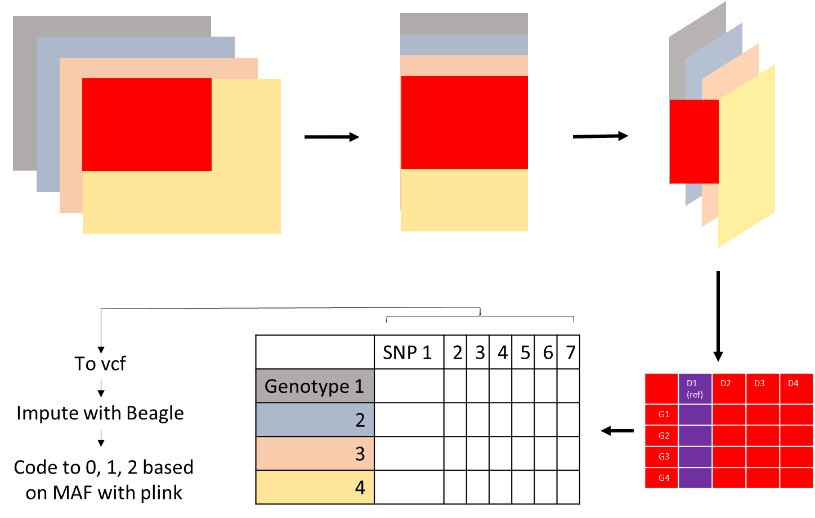
\includegraphics[width=0.75\textwidth]{pipeline_marker}
    \caption{Outlines of the steps in merging the chips. Four chips colored grey to yellow are used for representation. For a subset of markers (indicated by red box), each marker was evaluated based on overlapping genotypes to correct for markers inversions and genotyping errors.}
    \label{fig_pipeline_marker}
\end{figure}

The integrated arrays were further filtered for markers with high missing values as well as low minor allele frequency. Lastly, the integrated data was converted to a .vcf format \cite{danecek2011variant} for subsequent imputation with beagle 5.2 \cite{browning2018one}.The downstream processing involved using vcftools \cite{danecek2011variant} and plink \cite{purcell2007plink} to convert the string data .vcf file into numeric data coded 0,1, 2 accordingly for the number of genotype reference alleles. The hybrid genotypes were deduced form the parent genotypic data and were appended to the integrated parent genotypic matrix.

\textit{Daily means of twenty-eight climate variables was used to derive environment kinship}

Daily climate data for 28 variables were obtained from KWS SAAT SE \& Co. KGaA and used to derive Environment covariables (ECs) to capture variations between environments. ECs were derived for each environment and were calculated as mean monthly values of 28 weather variables starting from 1st October of the respective year of an environment and ending on 31st August in the following year.

The environment relationship matrix (\textit{ERM}) was then calculated as:

\vspace{6pt}

\begin{equation}
\hspace{0.5cm}\textit{ERM}_l = EC \cdot EC^T
\end{equation}

\vspace{6pt}

\begin{equation}
\hspace{0.5cm}\textit{ERM}_{nl} = \exp\left(\frac{{\text{dist}(EC)}}{\theta}\right)
\end{equation}

\vspace{6pt}

where EC is the scaled Environment covariate matrix, $EC^T$ is the transpose of the EC matrix, $\text{dist}(EC)$ is the Euclidean Distance matrix of EC, and $\theta$ is a scaling factor.

The $\textit{ERM}_l$ matrix is a proxy for kinship between respective environments, while the $\textit{ERM}_nl$ matrix builds upon it and represents a Gaussian kernel for environmental effects.

\textit{Integration of phenotypic, genotypic, and environment data was done to prepare the data for benchmarking with cross-validation scenarios.}

Two broad cases for grain yield prediction were considered. Firstly, prediction of mean genotypic values across environments, and secondly, prediction of mean genotypic values within environments. For the first case, only genotypic data was used as an input, whereas for the second case, genotypic data along with environment data was used as an input. Additionally, GxE data was approximated following \cite{de2020data}.

\textit{Dynamic CNN models were developed to benchmark against BLUP-based models.}

For the first case, i.e., prediction of mean genotypic values across environments, E-GBLUP incorporating an additive*additive epistasis matrix \cite{jiang2015modeling} was compared to a Convolutional Neural Network (CNN). Preliminary investigations with a static CNN revealed that relationships between the training and test datasets were poorly captured. Therefore, a dynamic Convolutional Neural Network with variable architectures derived specifically for each test-train split was developed. The CNN architectures were derived using the hyperband optimization algorithm \cite{li_hyperband_2018}. For CNN, a validation set was additionally created by subsetting 20\% from the respective train and test sets. The training and validation sets were used for hyperparameter tuning as well as learning weights and biases to produce a learned model for a given run. Grain yield values of the genotypes in the test population were then predicted.

The BLUEs (Best Linear Unbiased Estimates) were used in several types of cross-validation procedures to evaluate model robustness for grain yield prediction. In each of the 25 cross-validation runs, a training set, a validation set, and a test population were defined. The following cross-validation scenarios were investigated:

\begin{itemize}
    \item Traditional cross-validation - Here, genotypes were randomly divided into a training and a test population in a ratio of 80:20.
    \item Stratified cross-validation - a proportionate 80\% of the genotypes from each experimental series were randomly selected for the training population and the remaining 20\% of genotypes were pooled to form the test population.
    \item Cross-validation to investigate the prediction accuracy as a function of training population size - To investigate the effect of using BigData on model prediction accuracy, six scenarios (Table 2) were designed with gradually increasing training population size. 
\end{itemize}

For the second case, i.e., prediction of mean genotypic values within environments, E-GBLUP was extended (referred to as Ex-GBLUP) to include environmental and GxE effects in addition to the effects of genotypes (Table 3). An all-CNN model was developed with multiple input streams feeding into a concatenation layer, followed by dense layers. Each stream corresponds to different model inputs, namely genomic data plus twenty-eight weather variables (Fig. 2). The hyperparameters of the all-CNN model were tuned using the hyperband optimization algorithm \cite{li_hyperband_2018}. For all-CNN, a validation set was additionally created by subsetting 20\% from the respective train and test sets. 

The following cross-validation scenarios were implemented:

\begin{itemize}
    \item CV1 - known genotypes in known environments
    \item CV2 - known genotypes in new environments
    \item CV3 - new genotypes in known environments
    \item CV4 - new genotypes in new environments
\end{itemize}

\section{Results}
\textit{The integrated genotypic data captures genetic groups between constituent populations} 

The robustness of genotypic data integration was assessed by examining the pairwise $F_{st}$ statistic between major population groups and utilizing the integrated data for genomic predictions of those groups. The Exp\textunderscore5 population, which included hybrids and parents from a wide cross of elite lines with genebank material, served as an outgroup (Fig. \ref{fig_fst_plot}). The observed genetic bifurcation aligns with biological expectations, as the remaining population groups primarily consisted of elite lines and hybrids resulting from crosses between elite lines.

\begin{figure}[h]
    \centering
    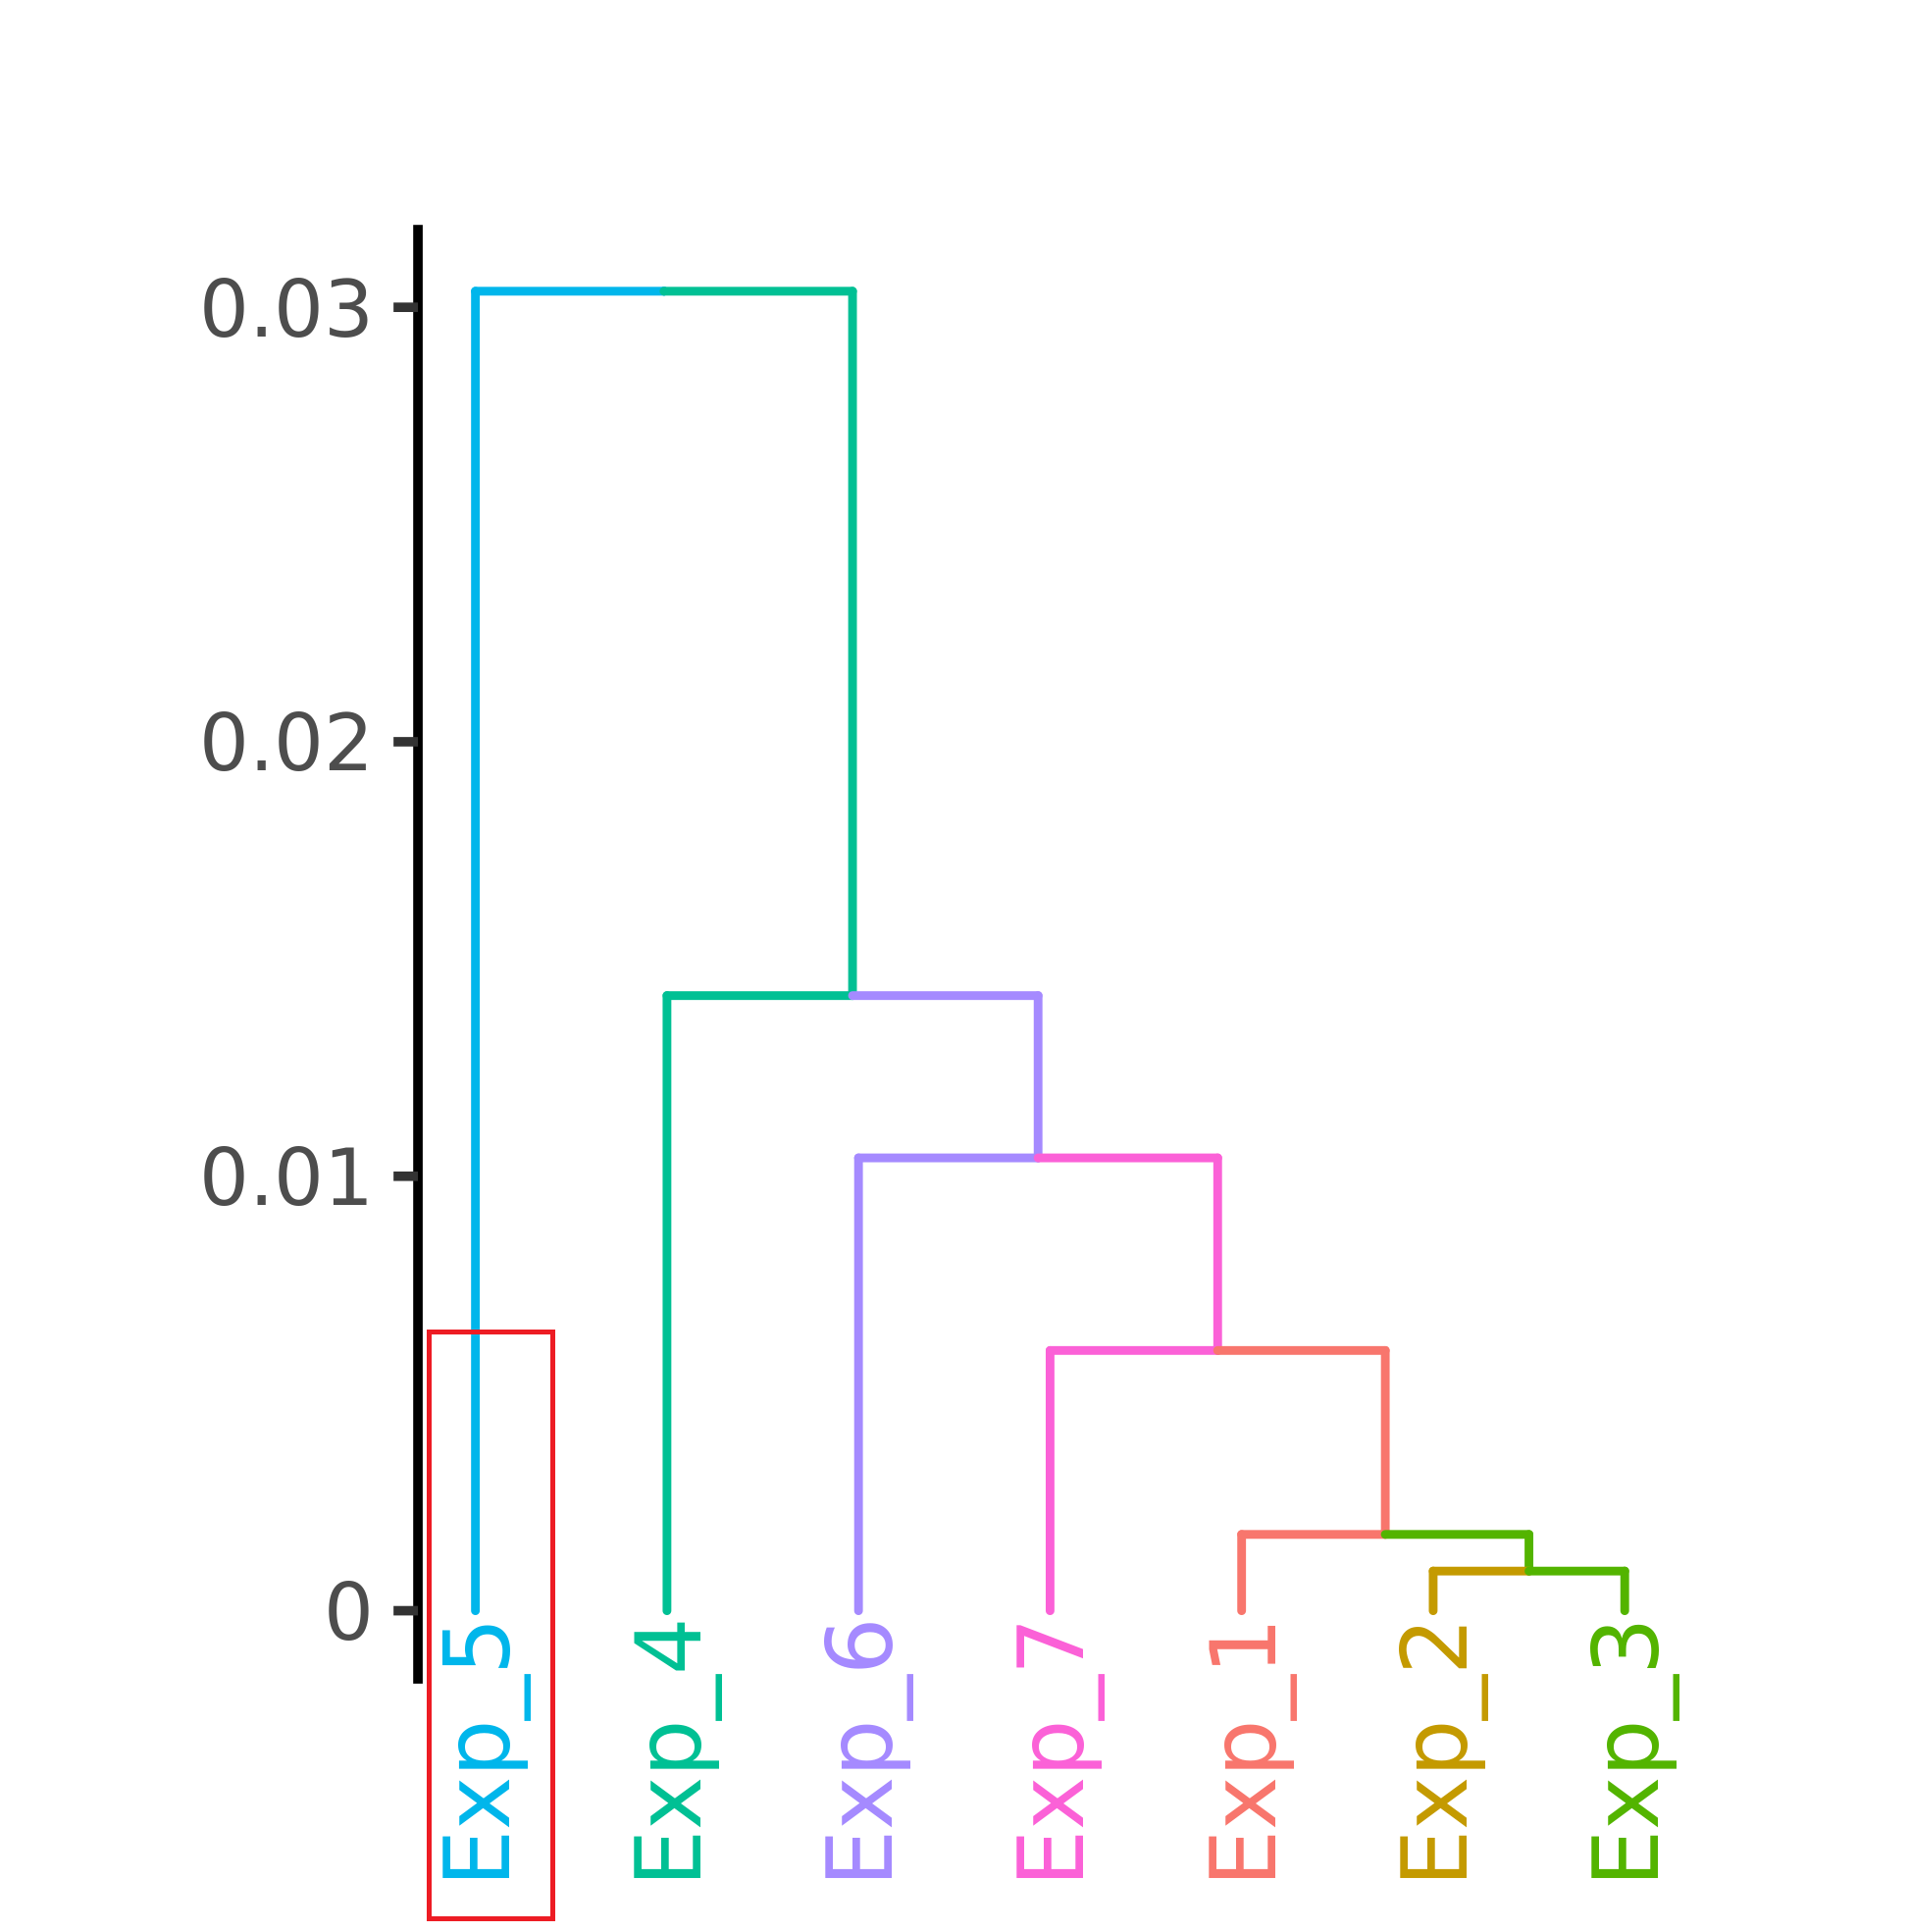
\includegraphics[width=0.5\textwidth]{fst_plot}
    \caption{$F_{st}$ statistic calculated between population groups indicate genetic divergence between the groups. The dendrogram was constructed by applying multidimensional scaling on pairwise $F_{st}$ matrix to show clustering between recently developed (outlined by the red box) and PGR derived population groups.}
    \label{fig_fst_plot}
\end{figure}

\textit{The environment relationship matrix reveals no environment relationship structure} 

The ERM was utilized to examine the presence of environmental clusters, but the analysis did not uncover any discernible pattern. This finding can be interpreted in two ways: 1. There are no environmental clusters present in the tested environments, or 2. There was an error in the calculation of the ERM. The latter possibility could be attributed to either poor-quality input data or an incorrect calculation method. However, since the data is sourced from a reliable pipeline, its quality is assured. To further investigate the calculation method, the ERM was computed using intervals of 5 and 10 days, in addition to the original 30-day interval. The null hypothesis, suggesting no relationship between ECs derived from the 5, 10, and 30-day intervals, was rejected based on the results of the \texttt{mantel.test()} function in R \cite{paradis_ape_2019}. Consequently, it was concluded that the examined environments lack any underlying structure and are truly diverse.

\textit{Dynamic CNN outperforms E-GBLUP for predicting average line grain yield} 

The performance of E-GBLUP and dynamic CNN models was benchmarked using three cross-validation scenarios. In the first scenario, traditional cross-validation was employed, where genotypes were randomly divided into a training and a test population in an 80:20 ratio. CNN model outperformed E-GBLUP for predicting line grain yield (Fig. \ref{fig_pred_corr_res_NN_2}). For the second scenario, stratified cross-validation was implemented to account for genetic distinctness observed in one experimental series (Fig. \ref{fig_pred_corr_res_NN_2}). The results showed slightly higher prediction accuracy in some cases compared to traditional cross-validation, but the overall trend of higher performance in case of lines was preserved here. The third scenario aimed to investigate the effect of utilizing BigData on prediction accuracy. Six scenarios were designed with gradually increasing training population sizes. The results demonstrated that as the training population size increased, the prediction accuracy improved, highlighting the utility of BigData for genomic prediction (Figure \ref{fig5}). Overall, Convolutional Neural Networks (CNN) exhibited superior performance compared to the traditional GBLUP based method, especially when dealing with extensive data or when flexibility in the genetic structure of training and test populations was required.

\begin{figure}[h]
    \centering
    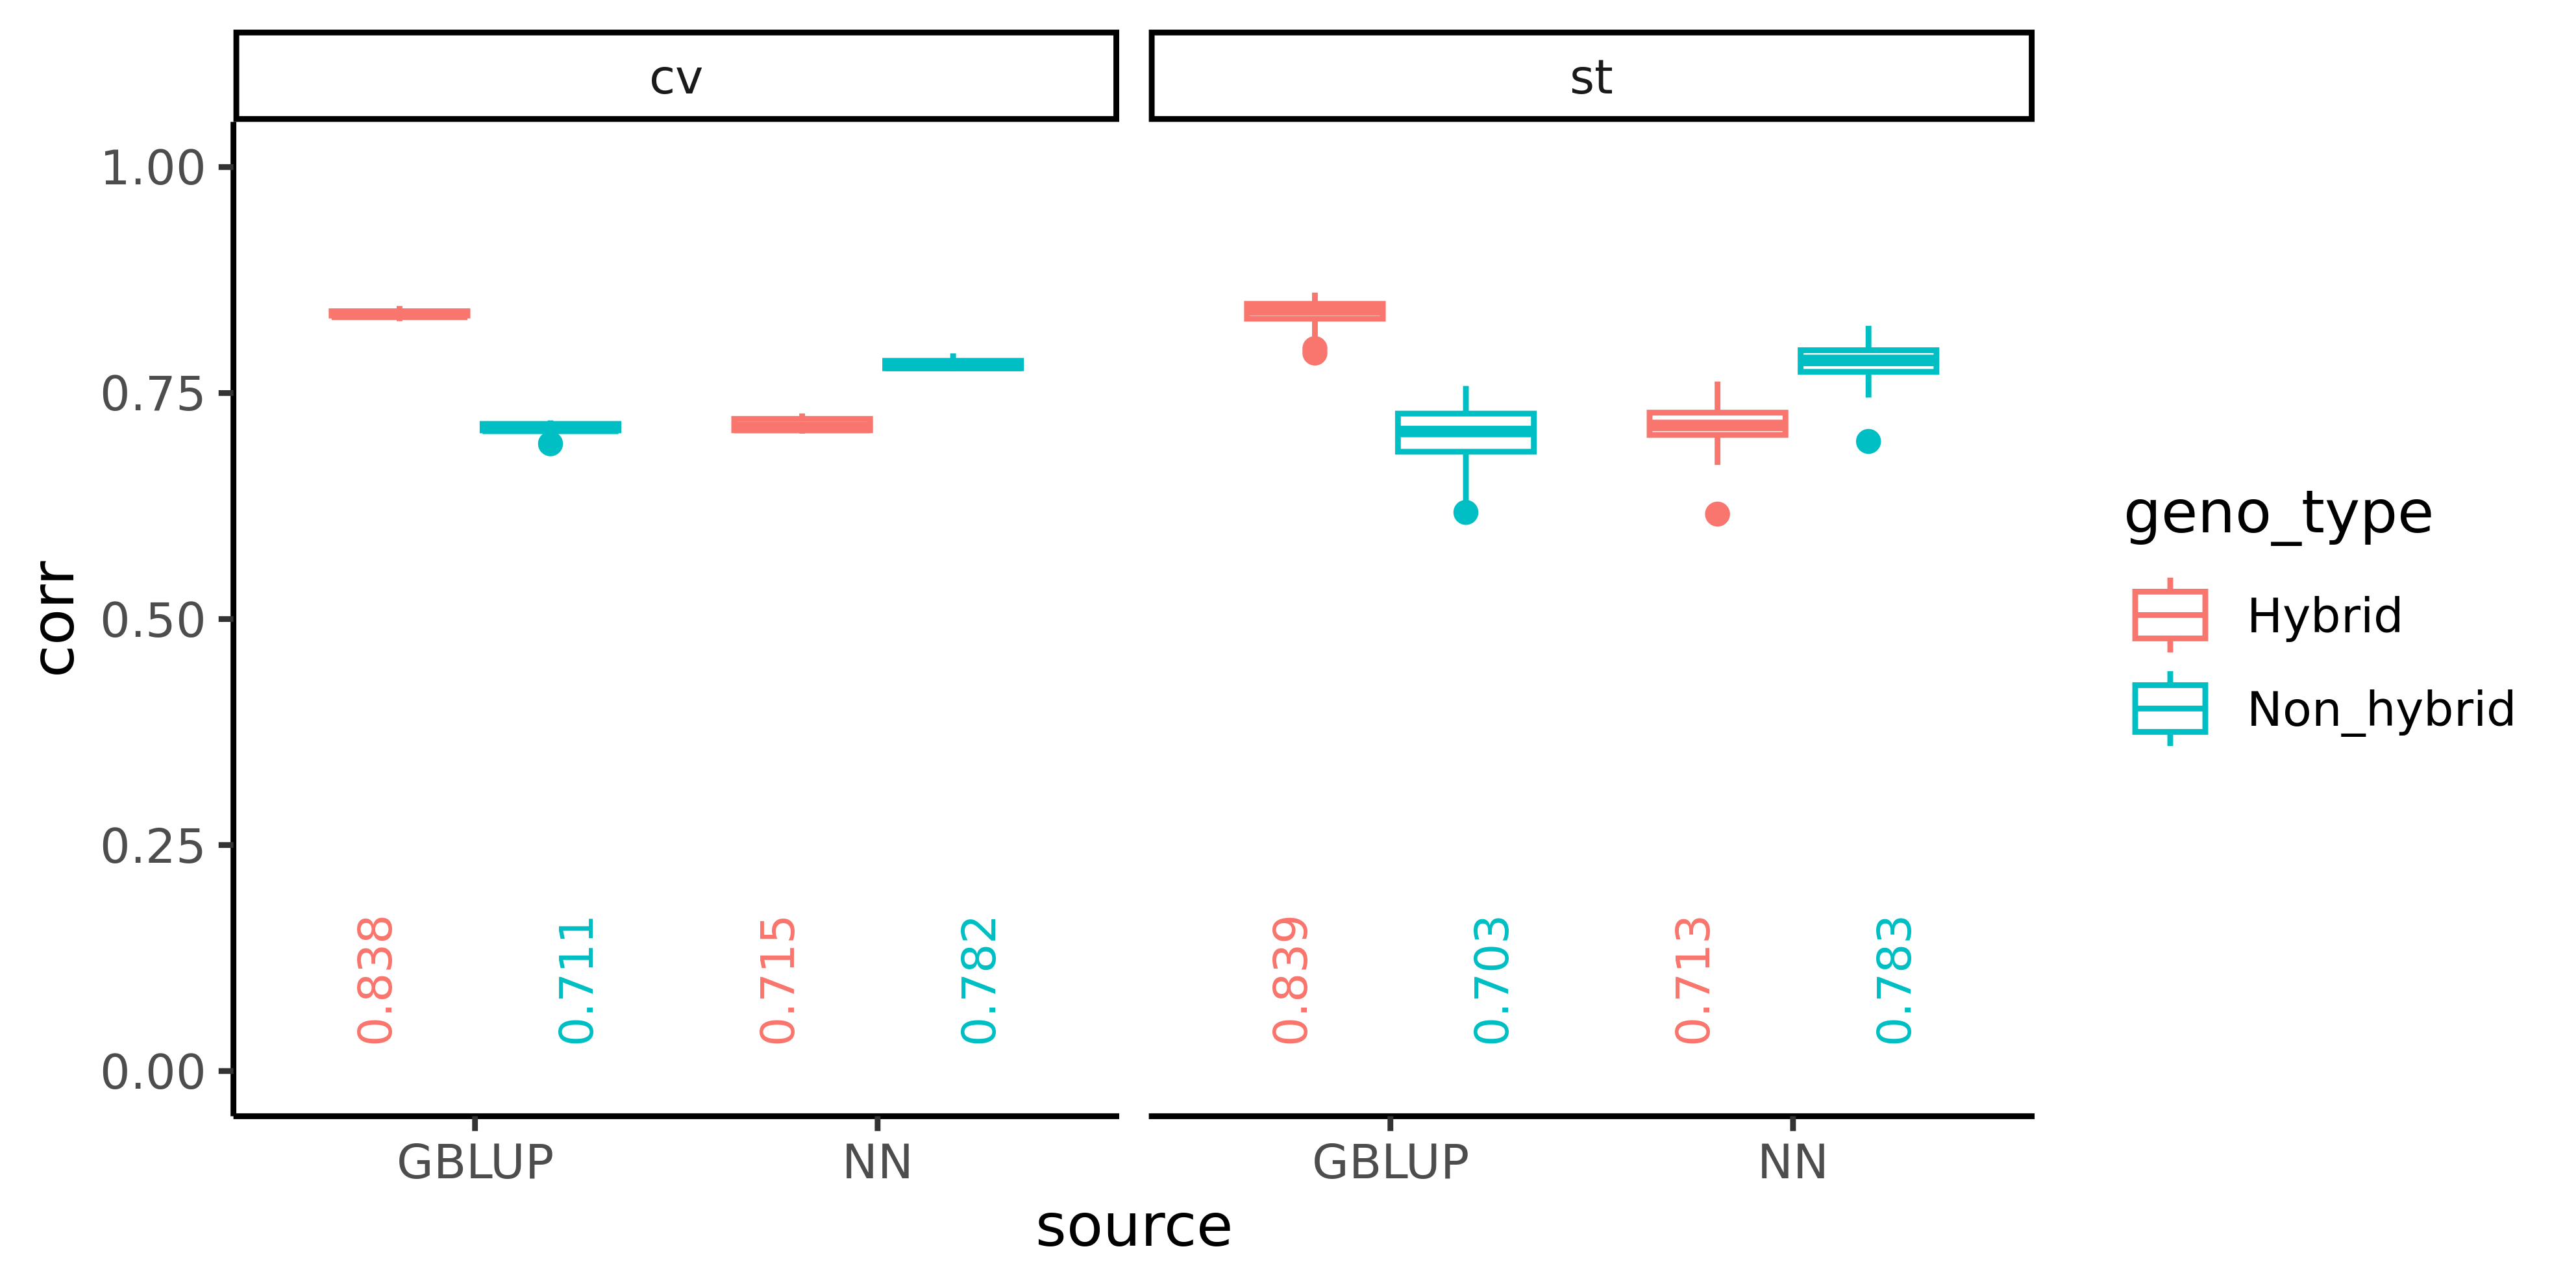
\includegraphics[width=0.9\textwidth]{pred_corr_res_NN_2}
    \caption{Genomic prediction accuracy (corr on y-axis between 0 to 1 ) of GBLUP and Convolutional Neural Networks (NN) for mean grain yield across sites under 5-fold cross validation (cv) and stratified cross validation (st). Results are shown separately for hybrids and lines.}
    \label{fig_pred_corr_res_NN_2}
\end{figure}

\textit{All-CNN benefits from increased training set size but fails to outperform Ex-GBLUP} 

The results from 25 cross-validation runs per combination of nine models and four scenarios are summarized in Figure \ref{fig6}. The findings indicate that models incorporating genomic and environmental relatedness consistently outperform those that ignore relatedness, except for CV2. Notably, the prediction accuracy for non-hybrid performance is consistently higher than that for hybrid performance across all scenarios. Complex models demonstrate superior performance in the CV3 and CV4 validation scenarios compared to other models. Specifically, model M5 and M6 exhibit similar performance trends, outperforming M4 in CV3 and CV4, while not showing the same advantage in CV1 and CV2. These results emphasize the importance of considering genomic and environmental relatedness in predictive

\section{Conclusions}

ToDo

\printbibliography%if you use biblatex/Biber
\end{document}